\documentclass[a4paper]{book}
\usepackage{makeidx}
\usepackage{natbib}
\usepackage{graphicx}
\usepackage{multicol}
\usepackage{float}
\usepackage{listings}
\usepackage{color}
\usepackage{ifthen}
\usepackage[table]{xcolor}
\usepackage{textcomp}
\usepackage{alltt}
\usepackage{ifpdf}
\ifpdf
\usepackage[pdftex,
            pagebackref=true,
            colorlinks=true,
            linkcolor=blue,
            unicode
           ]{hyperref}
\else
\usepackage[ps2pdf,
            pagebackref=true,
            colorlinks=true,
            linkcolor=blue,
            unicode
           ]{hyperref}
\usepackage{pspicture}
\fi
\usepackage[utf8]{inputenc}
\usepackage{mathptmx}
\usepackage[scaled=.90]{helvet}
\usepackage{courier}
\usepackage{sectsty}
\usepackage[titles]{tocloft}
\usepackage{doxygen}
\lstset{language=C++,inputencoding=utf8,basicstyle=\footnotesize,breaklines=true,breakatwhitespace=true,tabsize=8,numbers=left }
\makeindex
\setcounter{tocdepth}{3}
\renewcommand{\footrulewidth}{0.4pt}
\renewcommand{\familydefault}{\sfdefault}
\hfuzz=15pt
\setlength{\emergencystretch}{15pt}
\hbadness=750
\tolerance=750
\begin{document}
\hypersetup{pageanchor=false,citecolor=blue}
\begin{titlepage}
\vspace*{7cm}
\begin{center}
{\Large \-Project \-Orwell \-Client \\[1ex]\large 1.\-0 }\\
\vspace*{1cm}
{\large \-Generated by Doxygen 1.7.5}\\
\vspace*{0.5cm}
{\small Fri May 4 2012 03:34:07}\\
\end{center}
\end{titlepage}
\clearemptydoublepage
\pagenumbering{roman}
\tableofcontents
\clearemptydoublepage
\pagenumbering{arabic}
\hypersetup{pageanchor=true,citecolor=blue}
\chapter{\-Namespace \-Index}
\section{\-Namespace \-List}
\-Here is a list of all documented namespaces with brief descriptions\-:\begin{DoxyCompactList}
\item\contentsline{section}{\hyperlink{namespaceapp_1_1Controller}{app$\backslash$\-Controller} }{\pageref{namespaceapp_1_1Controller}}{}
\item\contentsline{section}{\hyperlink{namespaceapp_1_1Model}{app$\backslash$\-Model} }{\pageref{namespaceapp_1_1Model}}{}
\end{DoxyCompactList}

\chapter{\-Class \-Index}
\section{\-Class \-Hierarchy}
\-This inheritance list is sorted roughly, but not completely, alphabetically\-:\begin{DoxyCompactList}
\item \contentsline{section}{\-App\-Controller}{\pageref{classAppController}}{}
\begin{DoxyCompactList}
\item \contentsline{section}{\-Documents\-Controller}{\pageref{classDocumentsController}}{}
\item \contentsline{section}{\-Hosts\-Controller}{\pageref{classHostsController}}{}
\item \contentsline{section}{\-Pages\-Controller}{\pageref{classPagesController}}{}
\item \contentsline{section}{\-Users\-Controller}{\pageref{classUsersController}}{}
\end{DoxyCompactList}
\item \contentsline{section}{\-App\-Model}{\pageref{classAppModel}}{}
\begin{DoxyCompactList}
\item \contentsline{section}{\-Document}{\pageref{classDocument}}{}
\item \contentsline{section}{\-Host}{\pageref{classHost}}{}
\item \contentsline{section}{\-User}{\pageref{classUser}}{}
\end{DoxyCompactList}
\end{DoxyCompactList}

\chapter{\-Class \-Index}
\section{\-Class \-List}
\-Here are the classes, structs, unions and interfaces with brief descriptions\-:\begin{DoxyCompactList}
\item\contentsline{section}{\hyperlink{classAppController}{\-App\-Controller} }{\pageref{classAppController}}{}
\item\contentsline{section}{\hyperlink{classAppModel}{\-App\-Model} }{\pageref{classAppModel}}{}
\item\contentsline{section}{\hyperlink{classDocument}{\-Document} }{\pageref{classDocument}}{}
\item\contentsline{section}{\hyperlink{classDocumentsController}{\-Documents\-Controller} }{\pageref{classDocumentsController}}{}
\item\contentsline{section}{\hyperlink{classHost}{\-Host} }{\pageref{classHost}}{}
\item\contentsline{section}{\hyperlink{classHostDocument}{\-Host\-Document} }{\pageref{classHostDocument}}{}
\item\contentsline{section}{\hyperlink{classHostsController}{\-Hosts\-Controller} }{\pageref{classHostsController}}{}
\item\contentsline{section}{\hyperlink{classPagesController}{\-Pages\-Controller} }{\pageref{classPagesController}}{}
\end{DoxyCompactList}

\chapter{\-File \-Index}
\section{\-File \-List}
\-Here is a list of all documented files with brief descriptions\-:\begin{DoxyCompactList}
\item\contentsline{section}{\hyperlink{AppController_8php}{\-App\-Controller.\-php} \\*\-Base controller inherited by other controllers }{\pageref{AppController_8php}}{}
\item\contentsline{section}{\hyperlink{AppModel_8php}{\-App\-Model.\-php} \\*\-Base model inherited by other models }{\pageref{AppModel_8php}}{}
\item\contentsline{section}{\hyperlink{Document_8php}{\-Document.\-php} \\*\-Model for documents }{\pageref{Document_8php}}{}
\item\contentsline{section}{\hyperlink{DocumentsController_8php}{\-Documents\-Controller.\-php} \\*\-Controller for document operations }{\pageref{DocumentsController_8php}}{}
\item\contentsline{section}{\hyperlink{Host_8php}{\-Host.\-php} \\*\-Model for hosts }{\pageref{Host_8php}}{}
\item\contentsline{section}{\hyperlink{HostsController_8php}{\-Hosts\-Controller.\-php} \\*\-Controller for host operations }{\pageref{HostsController_8php}}{}
\item\contentsline{section}{\hyperlink{User_8php}{\-User.\-php} \\*\-Model for users }{\pageref{User_8php}}{}
\item\contentsline{section}{\hyperlink{UsersController_8php}{\-Users\-Controller.\-php} \\*\-Controller for user operations }{\pageref{UsersController_8php}}{}
\end{DoxyCompactList}

\chapter{\-Namespace \-Documentation}
\hypertarget{namespaceapp_1_1Controller}{
\section{app$\backslash$\-Controller \-Namespace \-Reference}
\label{namespaceapp_1_1Controller}\index{app$\backslash$\-Controller@{app$\backslash$\-Controller}}
}


\subsection{\-Detailed \-Description}
\-Static content controller

\-Override this controller by placing a copy in controllers directory of an application

\hyperlink{}{http\-://book.\-cakephp.\-org/2.\-0/en/controllers/pages-\/controller.\-html}
\hypertarget{namespaceapp_1_1Model}{
\section{app$\backslash$\-Model \-Namespace \-Reference}
\label{namespaceapp_1_1Model}\index{app$\backslash$\-Model@{app$\backslash$\-Model}}
}


\subsection{\-Detailed \-Description}
\-Application model for \-Cake.

\-This file is application-\/wide model file. \-You can put all application-\/wide model-\/related methods here.

\-P\-H\-P 5

\-Cake\-P\-H\-P(tm) \-: \-Rapid \-Development \-Framework (\href{http://cakephp.org}{\tt http\-://cakephp.\-org}) \-Copyright 2005-\/2011, \-Cake \-Software \-Foundation, \-Inc. (\href{http://cakefoundation.org}{\tt http\-://cakefoundation.\-org})

\-Licensed under \-The \-M\-I\-T \-License \-Redistributions of files must retain the above copyright notice.

\begin{DoxyCopyright}{\-Copyright}
\-Copyright 2005-\/2011, \-Cake \-Software \-Foundation, \-Inc. (\href{http://cakefoundation.org}{\tt http\-://cakefoundation.\-org}) \hyperlink{}{\-Cake\-P\-H\-P(tm) \-Project   \-Cake\-P\-H\-P(tm) v 0.\-2.\-9  \-M\-I\-T \-License (\href{http://www.opensource.org/licenses/mit-license.php}{\tt http\-://www.\-opensource.\-org/licenses/mit-\/license.\-php})  \-Application model for \-Cake.  \-Add your application-\/wide methods in the class below, your models will inherit them. }
\end{DoxyCopyright}

\chapter{\-Class \-Documentation}
\hypertarget{classAppController}{
\section{\-App\-Controller \-Class \-Reference}
\label{classAppController}\index{\-App\-Controller@{\-App\-Controller}}
}
\-Inheritance diagram for \-App\-Controller\-:\begin{figure}[H]
\begin{center}
\leavevmode
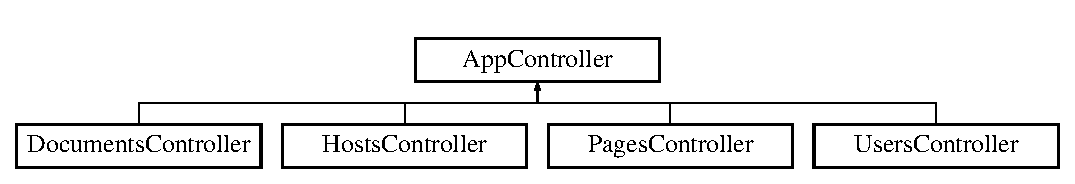
\includegraphics[height=2.000000cm]{classAppController}
\end{center}
\end{figure}
\subsection*{\-Public \-Member \-Functions}
\begin{DoxyCompactItemize}
\item 
\hypertarget{classAppController_ae6932ff72664b2b2a7f0bffc3e7f9bc7}{
{\bfseries before\-Filter} ()}
\label{classAppController_ae6932ff72664b2b2a7f0bffc3e7f9bc7}

\end{DoxyCompactItemize}
\subsection*{\-Public \-Attributes}
\begin{DoxyCompactItemize}
\item 
\hypertarget{classAppController_a7669889becf882a2fc3072131f0143e1}{
const {\bfseries \-S\-A\-L\-T} = '\-Zi\-Tt\-Ra\-In42'}
\label{classAppController_a7669889becf882a2fc3072131f0143e1}

\end{DoxyCompactItemize}


\-The documentation for this class was generated from the following file\-:\begin{DoxyCompactItemize}
\item 
\hyperlink{AppController_8php}{\-App\-Controller.\-php}\end{DoxyCompactItemize}

\hypertarget{classAppModel}{
\section{\-App\-Model \-Class \-Reference}
\label{classAppModel}\index{\-App\-Model@{\-App\-Model}}
}
\-Inheritance diagram for \-App\-Model\-:\begin{figure}[H]
\begin{center}
\leavevmode
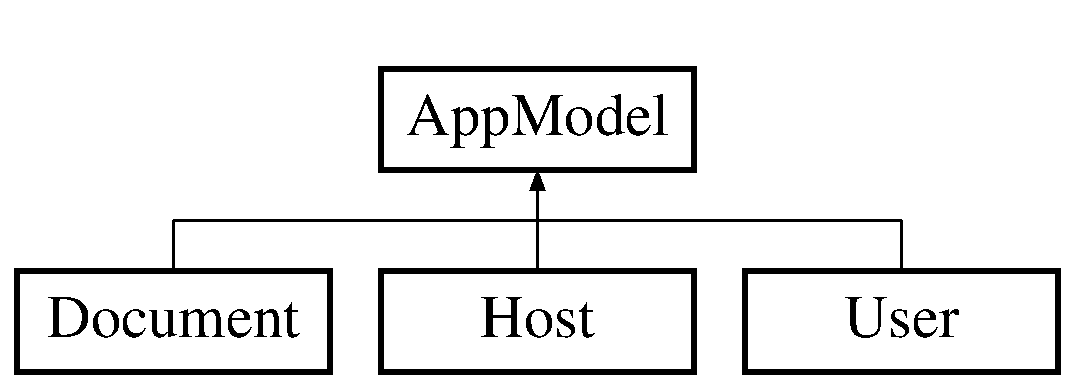
\includegraphics[height=2.000000cm]{classAppModel}
\end{center}
\end{figure}


\-The documentation for this class was generated from the following file\-:\begin{DoxyCompactItemize}
\item 
\hyperlink{AppModel_8php}{\-App\-Model.\-php}\end{DoxyCompactItemize}

\hypertarget{classDocument}{
\section{\-Document \-Class \-Reference}
\label{classDocument}\index{\-Document@{\-Document}}
}
\-Inheritance diagram for \-Document\-:\begin{figure}[H]
\begin{center}
\leavevmode
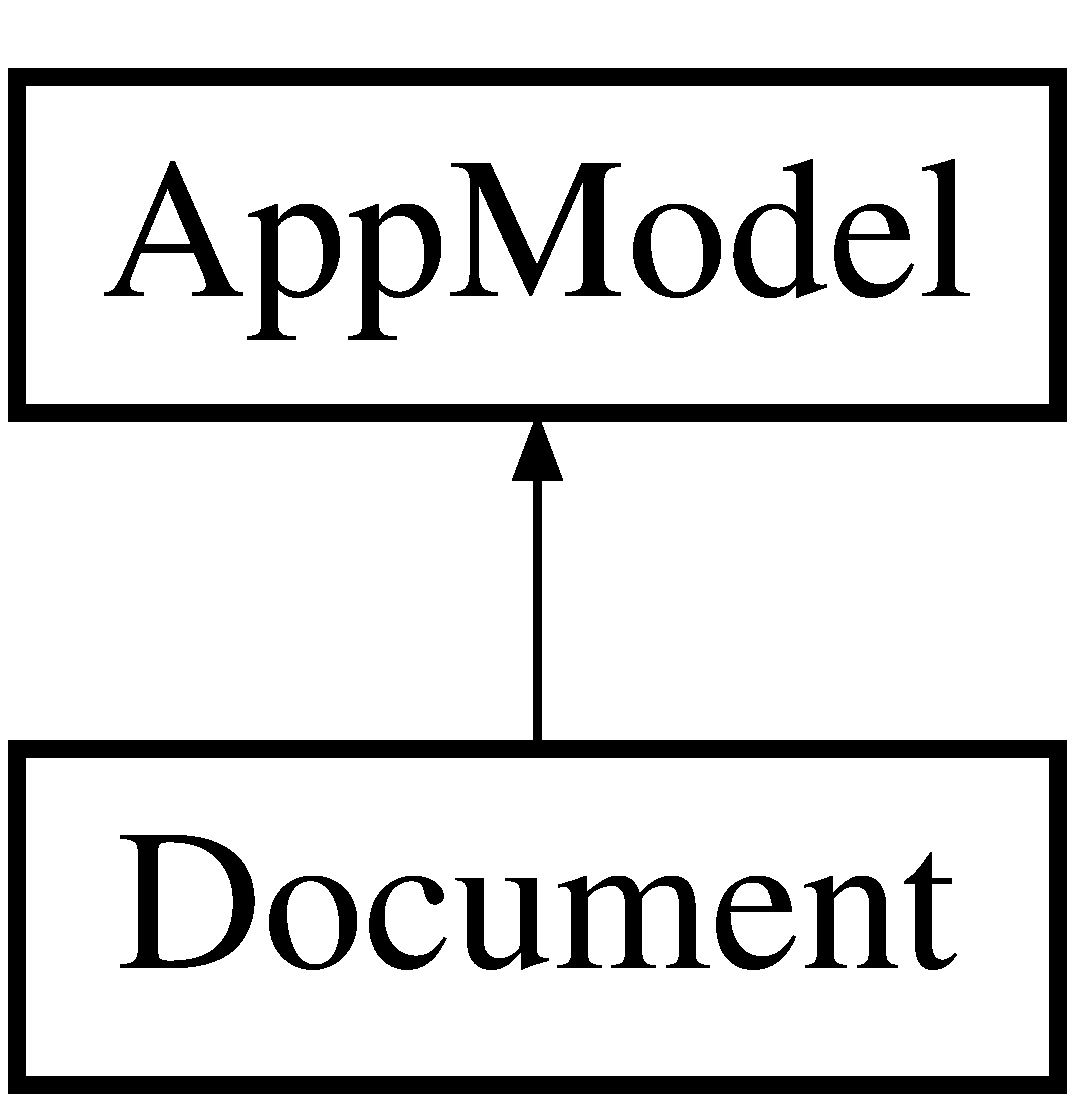
\includegraphics[height=2.000000cm]{classDocument}
\end{center}
\end{figure}


\-The documentation for this class was generated from the following file\-:\begin{DoxyCompactItemize}
\item 
\hyperlink{Document_8php}{\-Document.\-php}\end{DoxyCompactItemize}

\hypertarget{classDocumentsController}{
\section{\-Documents\-Controller \-Class \-Reference}
\label{classDocumentsController}\index{\-Documents\-Controller@{\-Documents\-Controller}}
}
\-Inheritance diagram for \-Documents\-Controller\-:\begin{figure}[H]
\begin{center}
\leavevmode
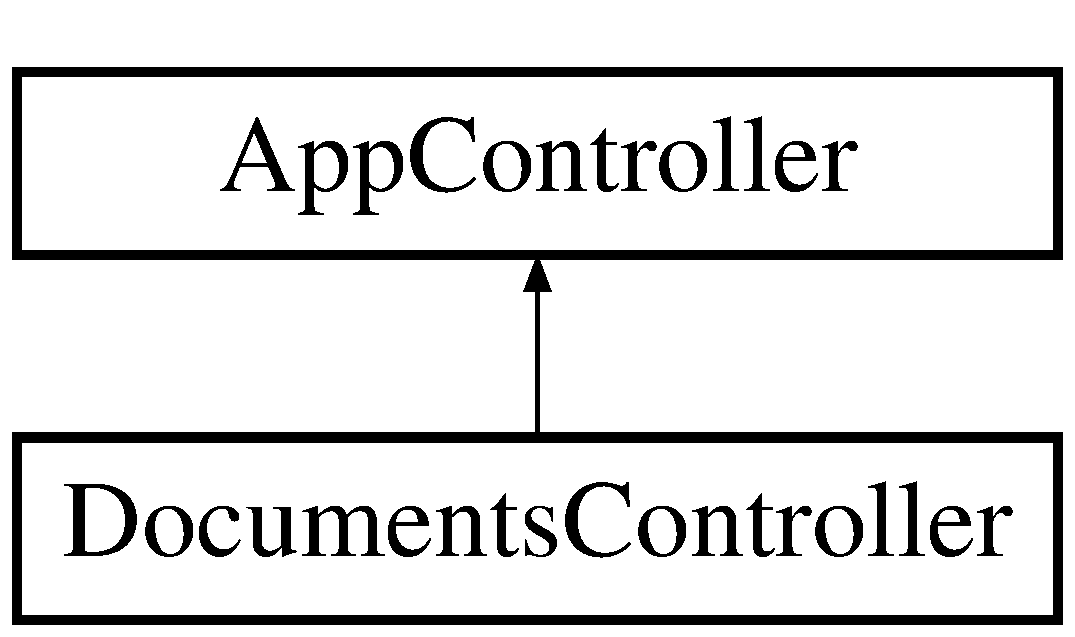
\includegraphics[height=2.000000cm]{classDocumentsController}
\end{center}
\end{figure}
\subsection*{\-Public \-Member \-Functions}
\begin{DoxyCompactItemize}
\item 
\hypertarget{classDocumentsController_ad4618f5bb5b8b51833956621b0071907}{
{\bfseries before\-Filter} ()}
\label{classDocumentsController_ad4618f5bb5b8b51833956621b0071907}

\item 
\hyperlink{classDocumentsController_ae9358b6908585ca36b92aa78afb657db}{add} ()
\item 
\hyperlink{classDocumentsController_ac01e57a9403d02d740e6e4fcce3e709b}{acquire} ()
\item 
\hyperlink{classDocumentsController_abe74e68167dd907c1e8428e399e10211}{browse} ()
\item 
\hyperlink{classDocumentsController_a44c8129ba74009effeaf9aa7add0d01f}{diff} (\$id)
\item 
\hyperlink{classDocumentsController_a5b77d80b7b2393a2b03202a9a50e02d7}{download} (\$id)
\item 
\hyperlink{classDocumentsController_acef7de0607f6c433bde6f1515e37d32f}{manage} ()
\item 
\hyperlink{classDocumentsController_a063eb26a98ab07696b2cde69f5c6a7f4}{repair} (\$id)
\item 
\hyperlink{classDocumentsController_a6ac7ef3b7865c256095065313cd7a87d}{snapshot} (\$id)
\item 
\hyperlink{classDocumentsController_adee0e3f5d87ba2bbc74a30ab4934bab7}{verify} (\$id=0)
\item 
\hyperlink{classDocumentsController_ad68485643e01e97a96f077d535865f05}{view} (\$id)
\end{DoxyCompactItemize}
\subsection*{\-Public \-Attributes}
\begin{DoxyCompactItemize}
\item 
\hypertarget{classDocumentsController_a6a79bec70bfcafa825c693be2971f618}{
{\bfseries \$require\-User} = array('add', 'browse', 'download', 'manage', 'repair')}
\label{classDocumentsController_a6a79bec70bfcafa825c693be2971f618}

\end{DoxyCompactItemize}


\subsection{\-Member \-Function \-Documentation}
\hypertarget{classDocumentsController_ac01e57a9403d02d740e6e4fcce3e709b}{
\index{\-Documents\-Controller@{\-Documents\-Controller}!acquire@{acquire}}
\index{acquire@{acquire}!DocumentsController@{\-Documents\-Controller}}
\subsubsection[{acquire}]{\setlength{\rightskip}{0pt plus 5cm}\-Documents\-Controller\-::acquire (
\begin{DoxyParamCaption}
{}
\end{DoxyParamCaption}
)}}
\label{classDocumentsController_ac01e57a9403d02d740e6e4fcce3e709b}
\-Wrapper for document acquisition method, checking api key first \hypertarget{classDocumentsController_ae9358b6908585ca36b92aa78afb657db}{
\index{\-Documents\-Controller@{\-Documents\-Controller}!add@{add}}
\index{add@{add}!DocumentsController@{\-Documents\-Controller}}
\subsubsection[{add}]{\setlength{\rightskip}{0pt plus 5cm}\-Documents\-Controller\-::add (
\begin{DoxyParamCaption}
{}
\end{DoxyParamCaption}
)}}
\label{classDocumentsController_ae9358b6908585ca36b92aa78afb657db}
\-Add a new document


\begin{DoxyParams}{\-Parameters}
{\em \$name} & \-Name of the document \\
\hline
\end{DoxyParams}
\hypertarget{classDocumentsController_abe74e68167dd907c1e8428e399e10211}{
\index{\-Documents\-Controller@{\-Documents\-Controller}!browse@{browse}}
\index{browse@{browse}!DocumentsController@{\-Documents\-Controller}}
\subsubsection[{browse}]{\setlength{\rightskip}{0pt plus 5cm}\-Documents\-Controller\-::browse (
\begin{DoxyParamCaption}
{}
\end{DoxyParamCaption}
)}}
\label{classDocumentsController_abe74e68167dd907c1e8428e399e10211}
\-Browse all documents on the central server \hypertarget{classDocumentsController_a44c8129ba74009effeaf9aa7add0d01f}{
\index{\-Documents\-Controller@{\-Documents\-Controller}!diff@{diff}}
\index{diff@{diff}!DocumentsController@{\-Documents\-Controller}}
\subsubsection[{diff}]{\setlength{\rightskip}{0pt plus 5cm}\-Documents\-Controller\-::diff (
\begin{DoxyParamCaption}
\item[{\$}]{id}
\end{DoxyParamCaption}
)}}
\label{classDocumentsController_a44c8129ba74009effeaf9aa7add0d01f}
\-Display the differences between two text files


\begin{DoxyParams}{\-Parameters}
{\em \$id} & \-I\-D of the locally-\/hosted document \\
\hline
{\em \$compare} & \-U\-R\-L of the document to compare to \\
\hline
\end{DoxyParams}
\hypertarget{classDocumentsController_a5b77d80b7b2393a2b03202a9a50e02d7}{
\index{\-Documents\-Controller@{\-Documents\-Controller}!download@{download}}
\index{download@{download}!DocumentsController@{\-Documents\-Controller}}
\subsubsection[{download}]{\setlength{\rightskip}{0pt plus 5cm}\-Documents\-Controller\-::download (
\begin{DoxyParamCaption}
\item[{\$}]{id}
\end{DoxyParamCaption}
)}}
\label{classDocumentsController_a5b77d80b7b2393a2b03202a9a50e02d7}
\-Download a document from the central server


\begin{DoxyParams}{\-Parameters}
{\em \$id} & \-I\-D of document to download \\
\hline
\end{DoxyParams}
\hypertarget{classDocumentsController_acef7de0607f6c433bde6f1515e37d32f}{
\index{\-Documents\-Controller@{\-Documents\-Controller}!manage@{manage}}
\index{manage@{manage}!DocumentsController@{\-Documents\-Controller}}
\subsubsection[{manage}]{\setlength{\rightskip}{0pt plus 5cm}\-Documents\-Controller\-::manage (
\begin{DoxyParamCaption}
{}
\end{DoxyParamCaption}
)}}
\label{classDocumentsController_acef7de0607f6c433bde6f1515e37d32f}
\-Manage documents \hypertarget{classDocumentsController_a063eb26a98ab07696b2cde69f5c6a7f4}{
\index{\-Documents\-Controller@{\-Documents\-Controller}!repair@{repair}}
\index{repair@{repair}!DocumentsController@{\-Documents\-Controller}}
\subsubsection[{repair}]{\setlength{\rightskip}{0pt plus 5cm}\-Documents\-Controller\-::repair (
\begin{DoxyParamCaption}
\item[{\$}]{id}
\end{DoxyParamCaption}
)}}
\label{classDocumentsController_a063eb26a98ab07696b2cde69f5c6a7f4}
\-Repair our document by downloading if from another host


\begin{DoxyParams}{\-Parameters}
{\em \$id} & \-I\-D of document to repair \\
\hline
{\em \$client} & \-Client from which to download document \\
\hline
\end{DoxyParams}
\hypertarget{classDocumentsController_a6ac7ef3b7865c256095065313cd7a87d}{
\index{\-Documents\-Controller@{\-Documents\-Controller}!snapshot@{snapshot}}
\index{snapshot@{snapshot}!DocumentsController@{\-Documents\-Controller}}
\subsubsection[{snapshot}]{\setlength{\rightskip}{0pt plus 5cm}\-Documents\-Controller\-::snapshot (
\begin{DoxyParamCaption}
\item[{\$}]{id}
\end{DoxyParamCaption}
)}}
\label{classDocumentsController_a6ac7ef3b7865c256095065313cd7a87d}
\-Create a snapshot of a document before it is verified


\begin{DoxyParams}{\-Parameters}
{\em \$id} & \-I\-D of document to snapshot \\
\hline
\end{DoxyParams}
\begin{DoxyReturn}{\-Returns}
\-Whether or not snapshot already existed 
\end{DoxyReturn}
\hypertarget{classDocumentsController_adee0e3f5d87ba2bbc74a30ab4934bab7}{
\index{\-Documents\-Controller@{\-Documents\-Controller}!verify@{verify}}
\index{verify@{verify}!DocumentsController@{\-Documents\-Controller}}
\subsubsection[{verify}]{\setlength{\rightskip}{0pt plus 5cm}\-Documents\-Controller\-::verify (
\begin{DoxyParamCaption}
\item[{\$}]{id = {\ttfamily 0}}
\end{DoxyParamCaption}
)}}
\label{classDocumentsController_adee0e3f5d87ba2bbc74a30ab4934bab7}
\-Verify the integrity of a single document


\begin{DoxyParams}{\-Parameters}
{\em \$id} & \-I\-D of document to verify. \-If not given, a random document is selected \\
\hline
\end{DoxyParams}
\hypertarget{classDocumentsController_ad68485643e01e97a96f077d535865f05}{
\index{\-Documents\-Controller@{\-Documents\-Controller}!view@{view}}
\index{view@{view}!DocumentsController@{\-Documents\-Controller}}
\subsubsection[{view}]{\setlength{\rightskip}{0pt plus 5cm}\-Documents\-Controller\-::view (
\begin{DoxyParamCaption}
\item[{\$}]{id}
\end{DoxyParamCaption}
)}}
\label{classDocumentsController_ad68485643e01e97a96f077d535865f05}
\-View a document hosted on the client


\begin{DoxyParams}{\-Parameters}
{\em \$id} & \-I\-D of document to view \\
\hline
\end{DoxyParams}


\-The documentation for this class was generated from the following file\-:\begin{DoxyCompactItemize}
\item 
\hyperlink{DocumentsController_8php}{\-Documents\-Controller.\-php}\end{DoxyCompactItemize}

\hypertarget{classHost}{
\section{\-Host \-Class \-Reference}
\label{classHost}\index{\-Host@{\-Host}}
}
\-Inheritance diagram for \-Host\-:\begin{figure}[H]
\begin{center}
\leavevmode
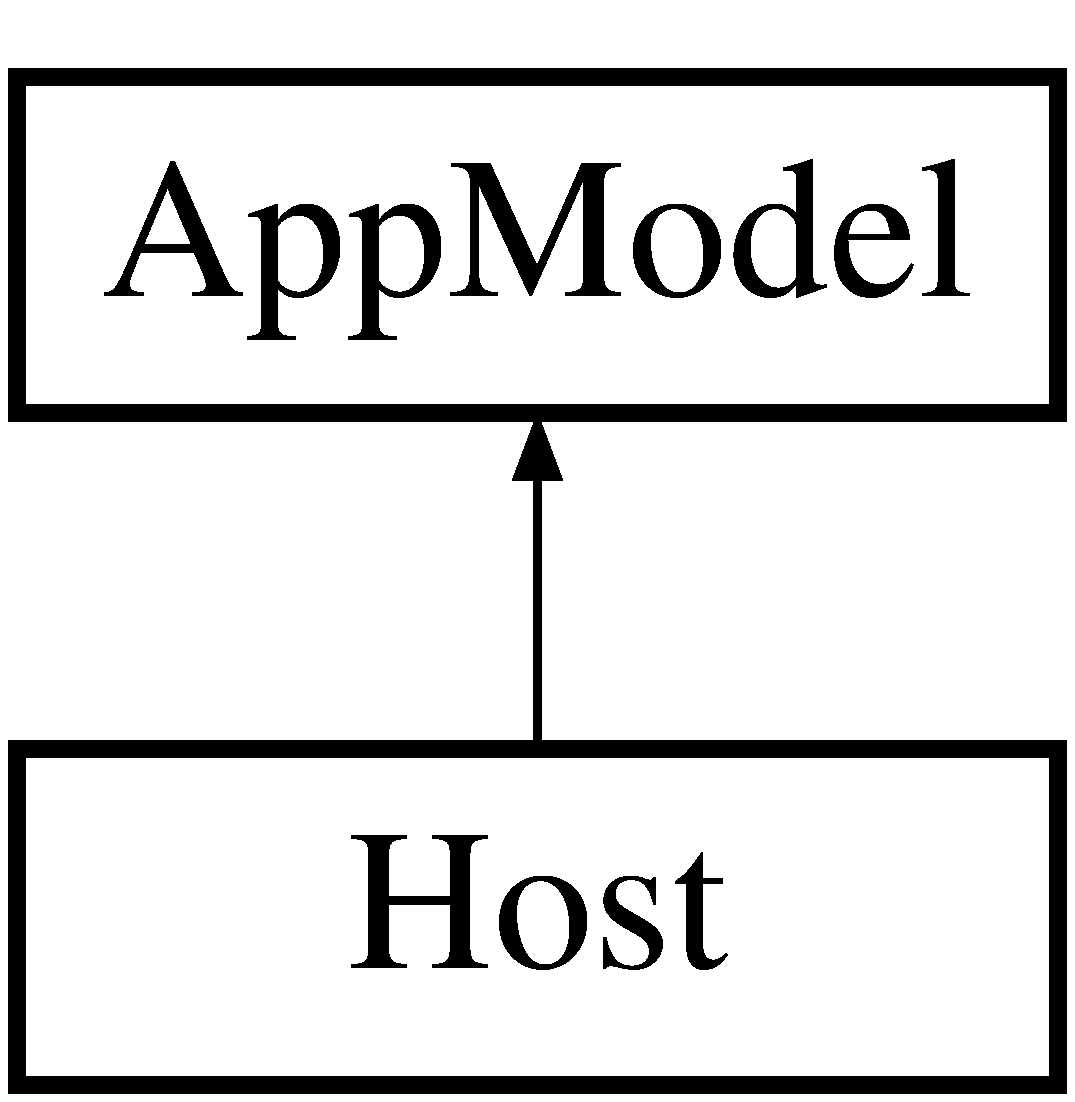
\includegraphics[height=2.000000cm]{classHost}
\end{center}
\end{figure}


\-The documentation for this class was generated from the following file\-:\begin{DoxyCompactItemize}
\item 
\hyperlink{Host_8php}{\-Host.\-php}\end{DoxyCompactItemize}

\hypertarget{classHostsController}{
\section{\-Hosts\-Controller \-Class \-Reference}
\label{classHostsController}\index{\-Hosts\-Controller@{\-Hosts\-Controller}}
}
\-Inheritance diagram for \-Hosts\-Controller\-:\begin{figure}[H]
\begin{center}
\leavevmode
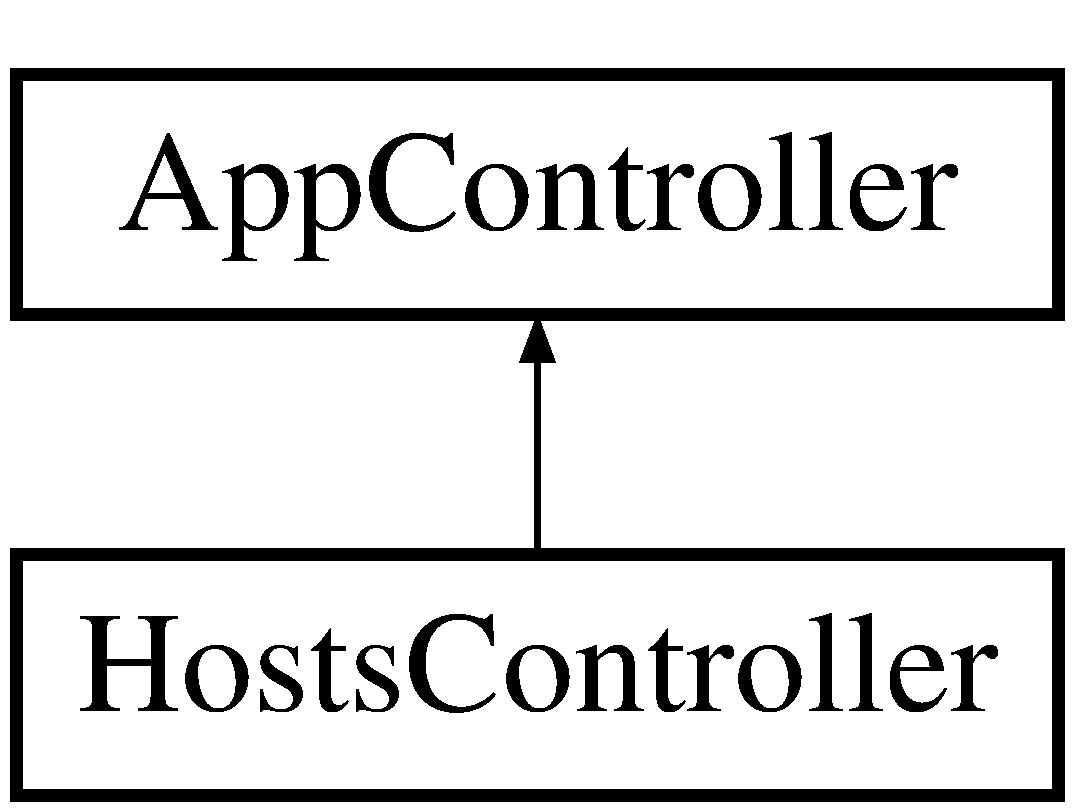
\includegraphics[height=2.000000cm]{classHostsController}
\end{center}
\end{figure}
\subsection*{\-Public \-Member \-Functions}
\begin{DoxyCompactItemize}
\item 
\hyperlink{classHostsController_a53995436c24d4b77cc3f7681c2487e6a}{add} ()
\item 
\hyperlink{classHostsController_ae1d16e1735d176e41b762701a48e657e}{notify} (\$document\-\_\-id)
\end{DoxyCompactItemize}


\subsection{\-Member \-Function \-Documentation}
\hypertarget{classHostsController_a53995436c24d4b77cc3f7681c2487e6a}{
\index{\-Hosts\-Controller@{\-Hosts\-Controller}!add@{add}}
\index{add@{add}!HostsController@{\-Hosts\-Controller}}
\subsubsection[{add}]{\setlength{\rightskip}{0pt plus 5cm}\-Hosts\-Controller\-::add (
\begin{DoxyParamCaption}
{}
\end{DoxyParamCaption}
)}}
\label{classHostsController_a53995436c24d4b77cc3f7681c2487e6a}
\-Add a host to a document


\begin{DoxyParams}{\-Parameters}
{\em \$url} & \-U\-R\-L of host to associate document with \\
\hline
{\em \$document\-\_\-id} & \-I\-D of document to associate with host \\
\hline
\end{DoxyParams}
\hypertarget{classHostsController_ae1d16e1735d176e41b762701a48e657e}{
\index{\-Hosts\-Controller@{\-Hosts\-Controller}!notify@{notify}}
\index{notify@{notify}!HostsController@{\-Hosts\-Controller}}
\subsubsection[{notify}]{\setlength{\rightskip}{0pt plus 5cm}\-Hosts\-Controller\-::notify (
\begin{DoxyParamCaption}
\item[{\$}]{document\-\_\-id}
\end{DoxyParamCaption}
)}}
\label{classHostsController_ae1d16e1735d176e41b762701a48e657e}
\-Notify a host that our document is correct


\begin{DoxyParams}{\-Parameters}
{\em \$document\-\_\-id} & \-I\-D of document in question \\
\hline
{\em \$compare} & \hyperlink{classHost}{\-Host} to notify regarding the integrity of the document \\
\hline
\end{DoxyParams}


\-The documentation for this class was generated from the following file\-:\begin{DoxyCompactItemize}
\item 
\hyperlink{HostsController_8php}{\-Hosts\-Controller.\-php}\end{DoxyCompactItemize}

\hypertarget{classPagesController}{
\section{\-Pages\-Controller \-Class \-Reference}
\label{classPagesController}\index{\-Pages\-Controller@{\-Pages\-Controller}}
}
\-Inheritance diagram for \-Pages\-Controller\-:\begin{figure}[H]
\begin{center}
\leavevmode
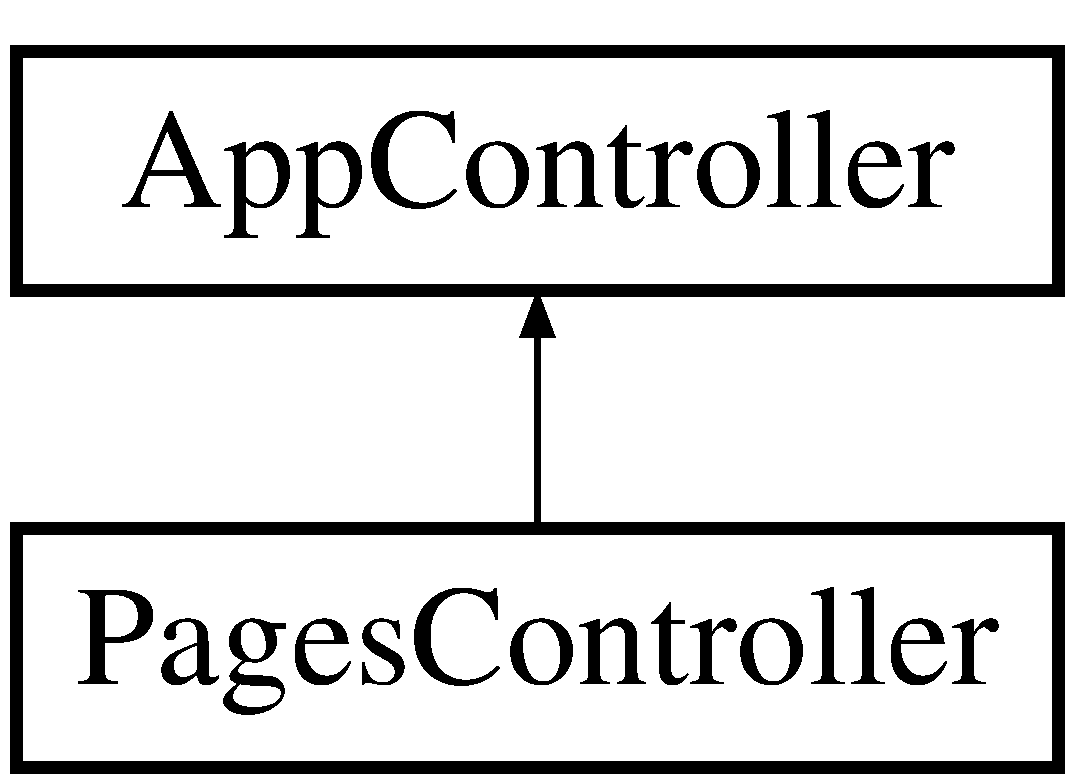
\includegraphics[height=2.000000cm]{classPagesController}
\end{center}
\end{figure}
\subsection*{\-Public \-Member \-Functions}
\begin{DoxyCompactItemize}
\item 
\hyperlink{classPagesController_a89f9b1e71fee5206f00be501df9c02e3}{display} ()
\end{DoxyCompactItemize}
\subsection*{\-Public \-Attributes}
\begin{DoxyCompactItemize}
\item 
\hypertarget{classPagesController_a8d4fa2edc8b67a9de41fd7cbf83faed0}{
{\bfseries \$name} = '\-Pages'}
\label{classPagesController_a8d4fa2edc8b67a9de41fd7cbf83faed0}

\item 
\hypertarget{classPagesController_a9dc3eac2482fd7925ed341208582c19a}{
{\bfseries \$helpers} = array('\-Html', '\-Session')}
\label{classPagesController_a9dc3eac2482fd7925ed341208582c19a}

\item 
\hypertarget{classPagesController_a75299c2f1604e1dba43af8f4234e4245}{
{\bfseries \$uses} = array()}
\label{classPagesController_a75299c2f1604e1dba43af8f4234e4245}

\end{DoxyCompactItemize}


\subsection{\-Member \-Function \-Documentation}
\hypertarget{classPagesController_a89f9b1e71fee5206f00be501df9c02e3}{
\index{\-Pages\-Controller@{\-Pages\-Controller}!display@{display}}
\index{display@{display}!PagesController@{\-Pages\-Controller}}
\subsubsection[{display}]{\setlength{\rightskip}{0pt plus 5cm}\-Pages\-Controller\-::display (
\begin{DoxyParamCaption}
{}
\end{DoxyParamCaption}
)}}
\label{classPagesController_a89f9b1e71fee5206f00be501df9c02e3}
\-Displays a view


\begin{DoxyParams}{\-Parameters}
{\em mixed} & \-What page to display \\
\hline
\end{DoxyParams}
\begin{DoxyReturn}{\-Returns}
void 
\end{DoxyReturn}


\-The documentation for this class was generated from the following file\-:\begin{DoxyCompactItemize}
\item 
\-Pages\-Controller.\-php\end{DoxyCompactItemize}

\hypertarget{classUser}{
\section{\-User \-Class \-Reference}
\label{classUser}\index{\-User@{\-User}}
}
\-Inheritance diagram for \-User\-:\begin{figure}[H]
\begin{center}
\leavevmode
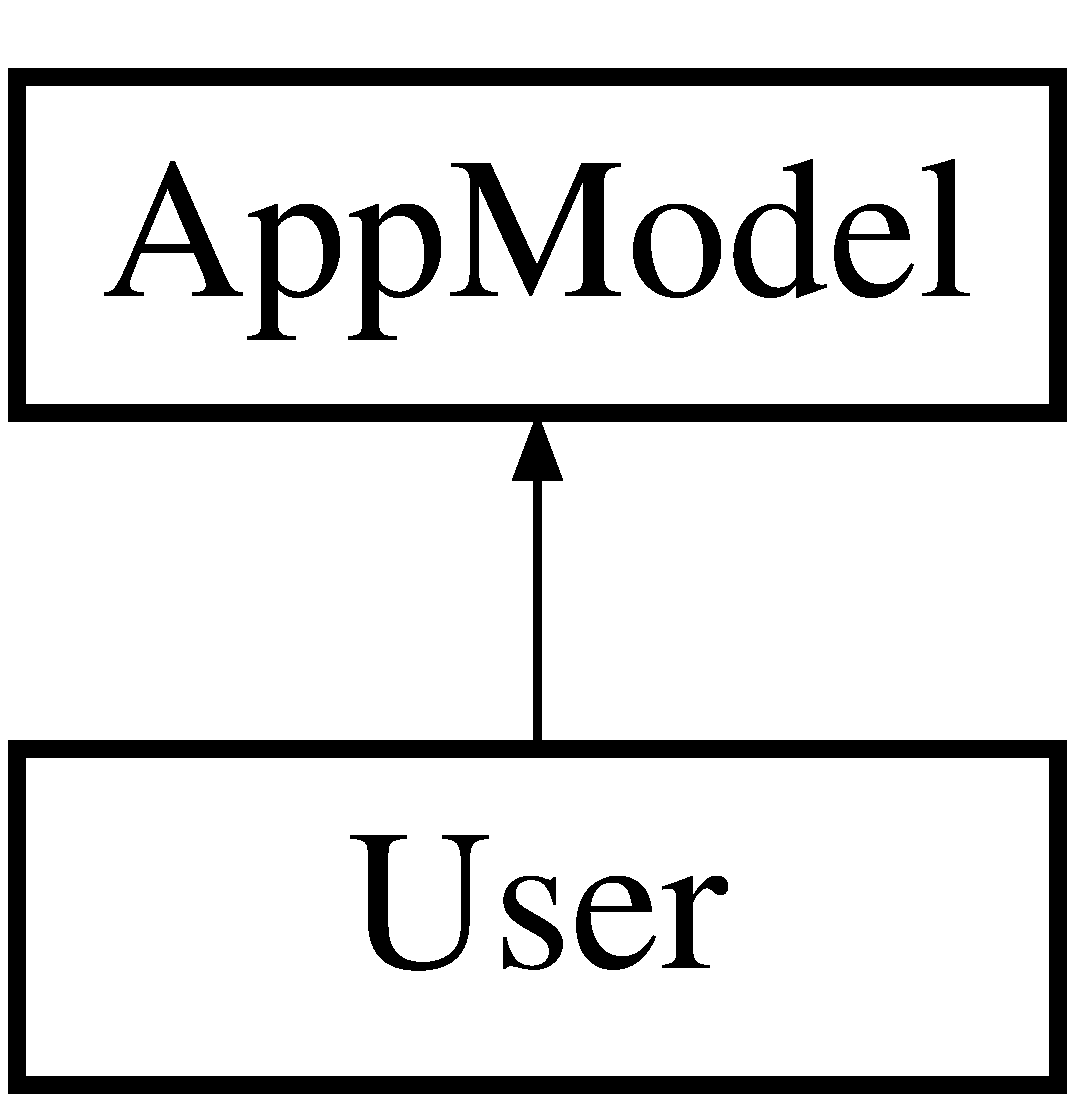
\includegraphics[height=2.000000cm]{classUser}
\end{center}
\end{figure}


\-The documentation for this class was generated from the following file\-:\begin{DoxyCompactItemize}
\item 
\hyperlink{User_8php}{\-User.\-php}\end{DoxyCompactItemize}

\hypertarget{classUsersController}{
\section{\-Users\-Controller \-Class \-Reference}
\label{classUsersController}\index{\-Users\-Controller@{\-Users\-Controller}}
}
\-Inheritance diagram for \-Users\-Controller\-:\begin{figure}[H]
\begin{center}
\leavevmode
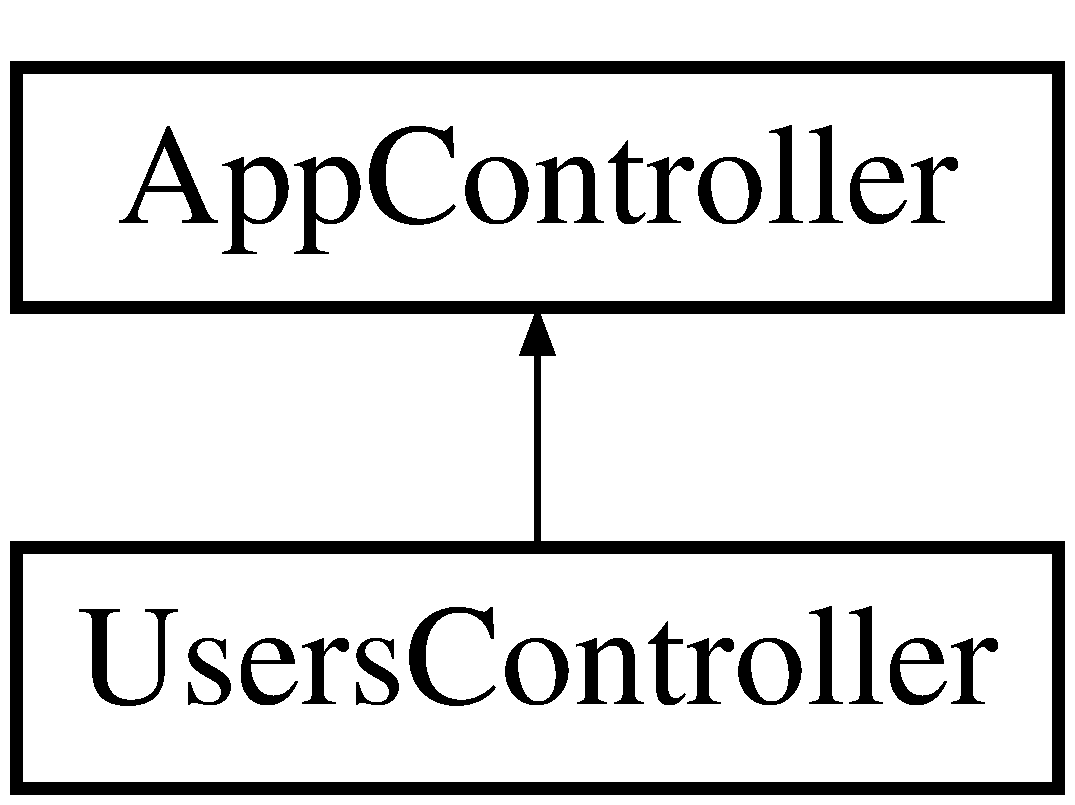
\includegraphics[height=2.000000cm]{classUsersController}
\end{center}
\end{figure}
\subsection*{\-Public \-Member \-Functions}
\begin{DoxyCompactItemize}
\item 
\hyperlink{classUsersController_aacebe6314e911b87dfb28785e87519cc}{login} ()
\item 
\hyperlink{classUsersController_abd5055ae74c89e431b061463ef7f2787}{logout} ()
\item 
\hyperlink{classUsersController_aff5905416e027604f61edcbe2cac2692}{register} ()
\end{DoxyCompactItemize}


\subsection{\-Member \-Function \-Documentation}
\hypertarget{classUsersController_aacebe6314e911b87dfb28785e87519cc}{
\index{\-Users\-Controller@{\-Users\-Controller}!login@{login}}
\index{login@{login}!UsersController@{\-Users\-Controller}}
\subsubsection[{login}]{\setlength{\rightskip}{0pt plus 5cm}\-Users\-Controller\-::login (
\begin{DoxyParamCaption}
{}
\end{DoxyParamCaption}
)}}
\label{classUsersController_aacebe6314e911b87dfb28785e87519cc}
\-Log the user in \hypertarget{classUsersController_abd5055ae74c89e431b061463ef7f2787}{
\index{\-Users\-Controller@{\-Users\-Controller}!logout@{logout}}
\index{logout@{logout}!UsersController@{\-Users\-Controller}}
\subsubsection[{logout}]{\setlength{\rightskip}{0pt plus 5cm}\-Users\-Controller\-::logout (
\begin{DoxyParamCaption}
{}
\end{DoxyParamCaption}
)}}
\label{classUsersController_abd5055ae74c89e431b061463ef7f2787}
\-Log the user out \hypertarget{classUsersController_aff5905416e027604f61edcbe2cac2692}{
\index{\-Users\-Controller@{\-Users\-Controller}!register@{register}}
\index{register@{register}!UsersController@{\-Users\-Controller}}
\subsubsection[{register}]{\setlength{\rightskip}{0pt plus 5cm}\-Users\-Controller\-::register (
\begin{DoxyParamCaption}
{}
\end{DoxyParamCaption}
)}}
\label{classUsersController_aff5905416e027604f61edcbe2cac2692}
\-Register a new user 

\-The documentation for this class was generated from the following file\-:\begin{DoxyCompactItemize}
\item 
\hyperlink{UsersController_8php}{\-Users\-Controller.\-php}\end{DoxyCompactItemize}

\chapter{\-File \-Documentation}
\hypertarget{AppController_8php}{
\section{\-App\-Controller.php \-File \-Reference}
\label{AppController_8php}\index{\-App\-Controller.\-php@{\-App\-Controller.\-php}}
}


\-Base controller inherited by other controllers.  


\subsection*{\-Classes}
\begin{DoxyCompactItemize}
\item 
class \hyperlink{classAppController}{\-App\-Controller}
\end{DoxyCompactItemize}


\subsection{\-Detailed \-Description}
\-Base controller inherited by other controllers. \begin{DoxyAuthor}{\-Author}
\-Tommy \-Mac\-William 
\end{DoxyAuthor}

\hypertarget{AppModel_8php}{
\section{\-App\-Model.php \-File \-Reference}
\label{AppModel_8php}\index{\-App\-Model.\-php@{\-App\-Model.\-php}}
}


\-Base model inherited by other models.  


\subsection*{\-Classes}
\begin{DoxyCompactItemize}
\item 
class \hyperlink{classAppModel}{\-App\-Model}
\end{DoxyCompactItemize}
\subsection*{\-Namespaces}
\begin{DoxyCompactItemize}
\item 
namespace \hyperlink{namespaceapp_1_1Model}{app$\backslash$\-Model}
\end{DoxyCompactItemize}


\subsection{\-Detailed \-Description}
\-Base model inherited by other models. \begin{DoxyAuthor}{\-Author}
\-Tommy \-Mac\-William 
\end{DoxyAuthor}

\hypertarget{Document_8php}{
\section{\-Document.php \-File \-Reference}
\label{Document_8php}\index{\-Document.\-php@{\-Document.\-php}}
}


\-Model for documents.  


\subsection*{\-Classes}
\begin{DoxyCompactItemize}
\item 
class \hyperlink{classDocument}{\-Document}
\end{DoxyCompactItemize}


\subsection{\-Detailed \-Description}
\-Model for documents. \begin{DoxyAuthor}{\-Author}
\-Tommy \-Mac\-William 
\end{DoxyAuthor}

\hypertarget{DocumentsController_8php}{
\section{\-Documents\-Controller.php \-File \-Reference}
\label{DocumentsController_8php}\index{\-Documents\-Controller.\-php@{\-Documents\-Controller.\-php}}
}


\-Controller for document operations.  


\subsection*{\-Classes}
\begin{DoxyCompactItemize}
\item 
class \hyperlink{classDocumentsController}{\-Documents\-Controller}
\end{DoxyCompactItemize}


\subsection{\-Detailed \-Description}
\-Controller for document operations. \begin{DoxyAuthor}{\-Author}
\-Tommy \-Mac\-William 
\end{DoxyAuthor}

\hypertarget{Host_8php}{
\section{\-Host.php \-File \-Reference}
\label{Host_8php}\index{\-Host.\-php@{\-Host.\-php}}
}


\-Model for hosts.  


\subsection*{\-Classes}
\begin{DoxyCompactItemize}
\item 
class \hyperlink{classHost}{\-Host}
\end{DoxyCompactItemize}


\subsection{\-Detailed \-Description}
\-Model for hosts. \begin{DoxyAuthor}{\-Author}
\-Tommy \-Mac\-William 
\end{DoxyAuthor}

\hypertarget{HostsController_8php}{
\section{\-Hosts\-Controller.php \-File \-Reference}
\label{HostsController_8php}\index{\-Hosts\-Controller.\-php@{\-Hosts\-Controller.\-php}}
}


\-Controller for host operations.  


\subsection*{\-Classes}
\begin{DoxyCompactItemize}
\item 
class \hyperlink{classHostsController}{\-Hosts\-Controller}
\end{DoxyCompactItemize}


\subsection{\-Detailed \-Description}
\-Controller for host operations. \begin{DoxyAuthor}{\-Author}
\-Tommy \-Mac\-William 
\end{DoxyAuthor}

\hypertarget{User_8php}{
\section{\-User.php \-File \-Reference}
\label{User_8php}\index{\-User.\-php@{\-User.\-php}}
}


\-Model for users.  


\subsection*{\-Classes}
\begin{DoxyCompactItemize}
\item 
class \hyperlink{classUser}{\-User}
\end{DoxyCompactItemize}


\subsection{\-Detailed \-Description}
\-Model for users. \begin{DoxyAuthor}{\-Author}
\-Tommy \-Mac\-William 
\end{DoxyAuthor}

\hypertarget{UsersController_8php}{
\section{\-Users\-Controller.php \-File \-Reference}
\label{UsersController_8php}\index{\-Users\-Controller.\-php@{\-Users\-Controller.\-php}}
}


\-Controller for user operations.  


\subsection*{\-Classes}
\begin{DoxyCompactItemize}
\item 
class \hyperlink{classUsersController}{\-Users\-Controller}
\end{DoxyCompactItemize}


\subsection{\-Detailed \-Description}
\-Controller for user operations. \begin{DoxyAuthor}{\-Author}
\-Tommy \-Mac\-William 
\end{DoxyAuthor}

\printindex
\end{document}
